\newsavebox{\smlmat}
\savebox{\smlmat}{$\smm{\bullet&\bullet\\\bullet& }$}
\newsavebox{\smlmatb}
\savebox{\smlmatb}{$\smm{\bullet&\bullet\\\bullet&\bullet}$}
\newsavebox{\smlmatc}
\savebox{\smlmatc}{$\smm{\bullet&\bullet&\bullet\\ &\bullet& }$}

\chapter{Characterizations}
\label{chap:chars}

\begin{defn}
A \emph{walk} in a matrix~$M$ is a sequence of some of its entries, beginning in the top left corner and ending in the bottom right one. If an entry $M[i,j]$ is in the sequence, the next one is either $M[i+1,j]$ or $M[i,j+1]$. Symmetrically, a \emph{reverse walk} in $M$ is a sequence of some of its entries, beginning in the top right corner and ending in the bottom left one.
\end{defn}

\begin{defn}
We call a matrix~$M$ a \emph{walking matrix} if there is a walk in $M$ such that all one-entries of $M$ are contained in the walk.
\end{defn}

\begin{defn}
For $M\in\Mat$ and $r\in[m],c\in[n]$ we say $M[r,c]$ is
\begin{itemize}
	\item \emph{top-left empty} if $M[[r-1],[c-1]]$ is an empty matrix,
	\item \emph{top-right empty} if $M[[r-1],[c+1,n]]$ is empty,
	\item \emph{bottom-left empty} if $M[[r-1],[c+1,n]]$ is empty,
	\item \emph{bottom-right empty} if $M[[r-1],[c+1,n]]$ is empty.
\end{itemize}
\end{defn}

\begin{defn}
For matrices $M\in\Mat$ and $M'\in\bin^{m\times l}$, we define $M\hsum M'\in\bin^{m\times(n+l)}$ to be the matrix created by extending $M$ by columns of $M'$.
\end{defn}

\section{Empty rows and columns}
\label{sec:empty}

\begin{obs}
\label{obs:emptyrows}
For a matrix $P\in\Pat$ let $P'=P\hsum 0^{k\times1}$, and for a matrix $M\in\Mat$ let $M'=M\hsum 1^{m\times1}$ then $\PimM\Leftrightarrow P'\im M'$.
\end{obs}
\begin{proof}
\begin{itemize}
	\item[$\Rightarrow$] We can map the last column of $P'$ just to the last column of $M'$ and then map $P'[[k],[l]]$ to $M'[[m],[n]]$ the same way $P$ is mapped to $M$.
	\item[$\Leftarrow$] We take the restriction of the mapping of $P'$ to $M'$ to get a mapping of $P$ to $M$.
\end{itemize}
\end{proof}

The same proof can be used for adding an empty column as the first column or an empty row as the first or the last row. Using induction we can easily show that a pattern $P'$ is avoided by a matrix $M'$ if and only if $P$ is avoided by $M$ where $P$ is derived from $P'$ by excluding all empty leading or ending rows and columns and $M$ is derived from $M'$ by excluding the same number of leading or ending rows and columns. Therefore, when characterizing matrices avoiding a forbidden pattern, we do not need to consider patterns having empty rows or columns on their boundary.

The following machinery shows what happens after we add empty columns in between two columns of a pattern that only has two columns.

\begin{defn}
For a matrix~$M\in\Mat$ a \emph{one-interval} is a sequence of consecutive one-entries in a single line of $M$ bounded by the edge of matrix or zero-entry from both sides.
\end{defn}

\begin{lemma}
\label{lemma:twocols}
Let $P\in\bin^{k\times2}$ and let $M\in\Mat$ be an inclusion maximal matrix avoiding $P$, then $M$ contains at most one one-interval in each row.
\end{lemma}
\begin{proof}
For contradiction, assume there are at least two one-intervals in a row of $M$. Because $M$ is inclusion maximal, changing any zero-entry~$e$ in between one-intervals $o_1$ and $o_2$ creates a mapping of the forbidden pattern. Such a mapping uses the changed one-entry to map an element $P[r',1]$ or $P[r',2]$.

In the first case, the same mapping also works if we use a one-entry from $o_1$ instead of $e$; thus, $\PnimM$ and we reach a contradiction. In the second case, the mapping can use a one-entry from $o_2$ instead of $e$; therefore, we again get a contradiction with $\PnimM$. Since $e$ is not usable for any one-entry of $P$, we can change it to a one-entry and get a contradiction with $M$ being inclusion maximal.
\end{proof}

\begin{lemma}
\label{lemma:maxmult}
Let $P\in\bin^{k\times2}$ and for any $l\geq1$ let $P^l\in\bin^{k\times(l+2)}$ be a pattern created from $P$ by adding $l$ new empty columns in between the two columns of $P$. If an $m\times n$ matrix $M\in\Avm{P^l}$ is inclusion maximal, then each row of $M$ is either empty or it contains a single one-interval of length at least $l+1$.
\end{lemma}
\begin{proof}
The same proof as in Lemma~\ref{lemma:twocols} shows that there is at most one one-interval in each row.

For contradiction, assume there are at most $l$ one-entries~$M[\{r\},[c_1,c_2]]$ in row~$r$:
\begin{itemize}
	\item $c_1=1$: we can set $M[r,c_2+1]=1$ and the matrix still avoids $P^l$, which is a contradiction with $M$ being inclusion maximal.
	\item $c_2=n$: we can set $M[r,c_1-1]=1$ and the matrix still avoids $P^l$, which is a contradiction with $M$ being inclusion maximal.
	\item otherwise: let us choose $e_l$ and $e_r$ zero-entries in row~$r$ such that there are exactly $l$ columns in between them and all one-entries of row~$r$ lie in between them. For contradiction, assume we cannot change neither $e_l=M[r,c_l]$ nor $e_r=M[r,c_r]$ to a one-entry without creating the pattern. This means $e_l$ is usable for some $P^l[r_1,1]$, let $m_l$ be the corresponding mapping. At the same time $e_r$ is usable for some $P^l[r_2,l+2]$ with $m_r$ being the corresponding mapping. We show that the two mappings can be combined to a mapping of $P^l$ to $M$ giving a contradiction. Without loss of generality, in both mappings, empty columns of $P$ are mapped exactly to $l$ columns of $M$. We describe how to partition $M$ into $k$ rows. Consider Figure~\ref{fig:emptymid}:
	\begin{itemize}
		\item $r_1\neq r_2$: Without loss of generality, we assume $r_1>r_2$. Let $r_3$ be the first row used to map $r_1$ in $m_l$ and let $r_4$ be the last row used to map $r_1$ in $m_r$. From $m_l$ being a mapping, we know that the first $r_1-1$ rows of $P$ can be mapped to rows $[1,r_3-1]$ of $M$ and from $m_r$ being a mapping, we know that the last $k-r_1$ rows of $P$ can be mapped to rows $[r_4+1,m]$ of $M$. Therefore, we can use rows $[r_3,r_4]$ of $M$ to map row~$r_1$ of $P$ without using one-entries $e_l$ and $e_r$.
		\item $r_1=r_2$: Let $r_3$ and $r_4$ be the first and the last rows respectively used to map $r_1$ in $m_l$ and let $r_5$ and $r_6$ be the first and the last rows respectively used to map $r_1$ in $m_r$. Without loss of generality let $r_3<r_5$. From $m_l$ being a mapping, we know that the first $r_1-1$ rows of $P$ can be mapped to rows $[1,r_3-1]$ of $M$. Without loss of generality let $r_4<r_6$. From $m_r$ being a mapping, we know that the last $k-r_1$ rows of $P$ can be mapped to rows $[r_6+1,m]$ of $M$. Therefore, we can use rows $[r_3,r_6]$ of $M$ to map row~$r_1$ of $P$ without using one-entries $e_l$ and $e_r$.
	\end{itemize}
\end{itemize}
We showed that either $e_l$ or $e_r$ can be changed to a one-entry, which is a contradiction with $M$ being inclusion maximal.

\begin{figure}[!ht]
\centering
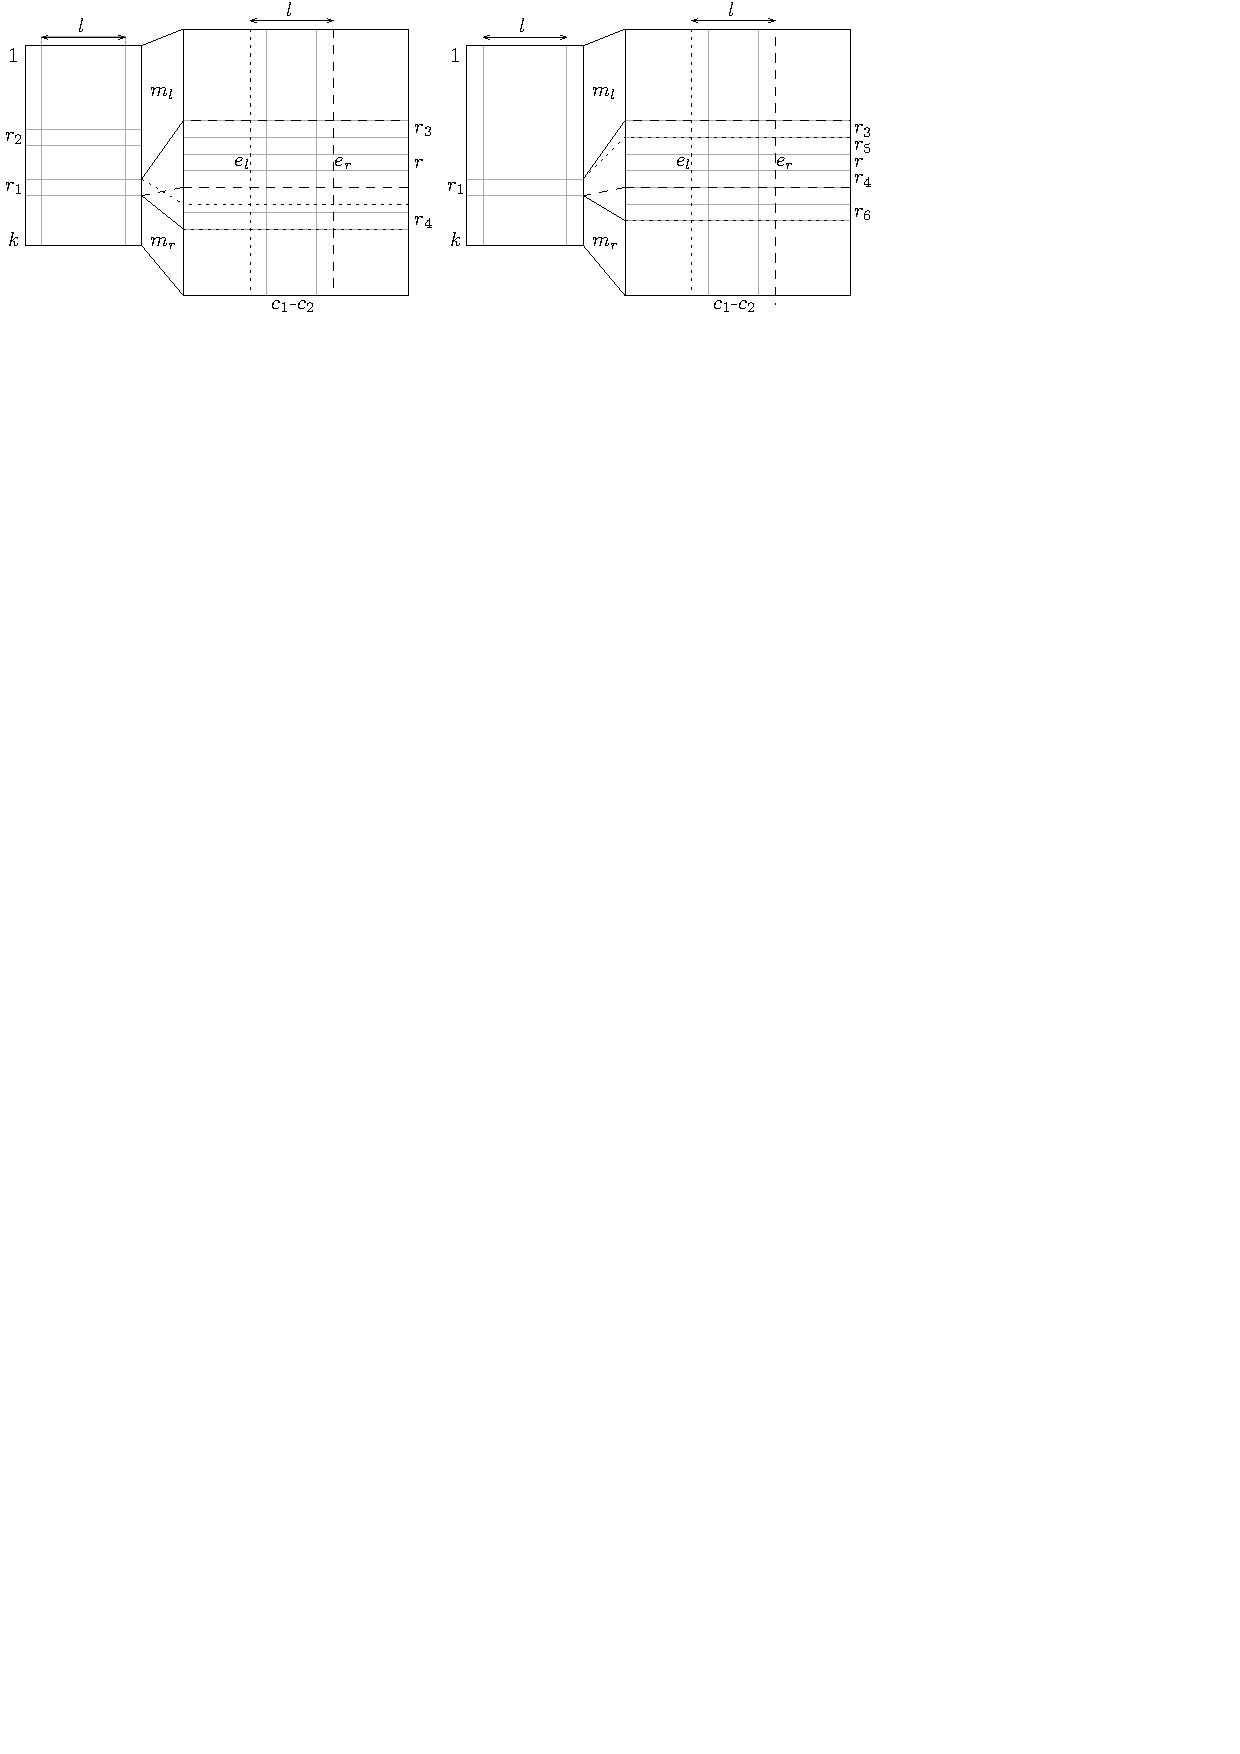
\includegraphics[width=\textwidth]{img/emptymid.pdf}
\caption{Dotted and dashed lines resembling mappings $m_l$ and $m_r$ of the forbidden pattern. Two horizontal lines show the boundaries of the mapping of row~$r$ and the vertical lines show boundaries of the mapping of column~$c$.}
\label{fig:emptymid}
\end{figure}
\end{proof}

\begin{thm}
\label{thm:emptymiddle}
Let $P\in\bin^{k\times2}$ and for any $l\geq1$ let $P^l\in\bin^{k\times(l+2)}$ be a pattern created from $P$ by adding $l$ new empty columns in between the two columns of $P$. For all $M\in\Mat$ it holds $M\in\Avm{P^l}\Leftrightarrow$ there exists $N\in\bin^{m\times(n-l)}$ such that $N\in\Avm{P}$ is inclusion maximal and $M$ is a submatrix of an elementwise OR of $N\hsum0^{m\times l},0^{m\times 1}\hsum N\hsum0^{m\times(l-1)},\dots,0^{m\times(l-1)}\hsum N\hsum0^{m\times1},0^{m\times l}\hsum N$.
\end{thm}
\begin{proof}
\begin{itemize}
	\item[$\Rightarrow$] It suffices to prove the statement for an inclusion maximal $M$. We know from Lemma~\ref{lemma:maxmult} that each row of $M$ contains either no one-entry or a single one-interval of length at least $l+1$. Let matrix $N$ be created from $M$ by deleting the last $l$ one-entries from each row and excluding the last $l$ columns. Clearly, $M$ is equal to an elementwise OR of $N\hsum0^{m\times l},0^{m\times 1}\hsum N\hsum0^{m\times(l-1)},\dots,0^{m\times(l-1)}\hsum N\hsum0^{m\times1},0^{m\times l}\hsum N$. If $P\im N$ then each mapping of $P$ can be extended to a mapping of $P^l$ to $M$ by mapping each $P^l[i,1]$ to the same one-entry where $P[i,1]$ is mapped in $N\hsum0^{m\times l}$ and mapping each $P^l[j,l+2]$ to the same one-entry where $P[j,2]$ is mapped in $0^{m\times l}\hsum N$.
	\item[$\Leftarrow$] Let $M$ be equal to an elementwise OR of $N\hsum0^{m\times l},0^{m\times 1}\hsum N\hsum0^{m\times(l-1)},\dots,0^{m\times(l-1)}\hsum N\hsum0^{m\times1},0^{m\times l}\hsum N$. For contradiction, assume $P^l\im M$ and consider any mapping of $P^l$ to $M$. Without loss of generality, one-entries of the first column of $P^l$ are mapped to those one-entries of $M$ created from $N\hsum0^{m\times l}$. If there is such one-entry mapped to a one-entry of $M$ not created from $N\hsum0^{m\times l}$, we just take the first one-entry in the row instead. Symmetrically, all one-entries of the last column of $P^l$ are mapped to one-entries created from $0^{m\times1}\hsum N$. The same one-entries of $N$ can be used to map $P$ to $N$, which is a contradiction.
\end{itemize}
\end{proof}

The same statement also holds when adding empty rows to a pattern that only has two rows. We can see in the following proposition that the straightforward generalization of the statement for bigger patterns does not hold.

\begin{prop}
There exists a matrix $P\in\Pat$ such that for each $P'\in\bin^{k\times(l+1)}$ created from $P$ by adding a single empty column in between two existing columns, there exists a matrix~$M\in\Mat$ such that $P'\im M$ and there exists $N\in\bin^{m\times(n-1)}$ such that $N\in\Avm{P}$ is inclusion maximal and $M$ is a submatrix of an elementwise OR of $N\hsum 0^{m\times 1}$ and $0^{m\times 1}\hsum N$.
\end{prop}
\begin{proof}
Later in this chapter, we characterize the class of matrices avoiding pattern~$P_8$. For the result, look at Proposition~\ref{prop:p72}. Let $N\in\Avm{P_8}$ be any matrix containing $P_5$ as an interval minor. Let $M$ be equal to $N\hsum 0^{m\times 1}$ placed over $0^{m\times 1}\hsum N$ with elementwise OR. Then $\smm{\bullet&\circ&\bullet&\bullet\\ &\circ&\bullet& },\smm{\bullet&\bullet&\circ&\bullet\\ &\bullet&\circ& }\im M$.
\end{proof}

Next, we characterize matrices avoiding some small patterns. Because of the above results, we also characterize some of their generalizations and we completely omit empty lines in them. If $\PnimM$ then also $P^T\nim M^T$ and this holds for all rotations and mirrors of $P$ and $M$ and so we only mention these symmetries and do not prove all characterizations one by one.

\section{Patterns having two one-entries and their generalization}
\label{sec:2ones}
These are, up to rotation and mirroring, the only patterns having two one-entries and no empty lines:
$$P_1=\smm{\bullet&\bullet}\ \ \ P_2=\smm{ &\bullet\\\bullet& }$$
They can be generalized to:
$$P'_1=\smm{\bullet&\cdots&\bullet}\ \ \ P'_2=\smm{ & &\bullet\\ &\cdots& \\\bullet& & }$$

\begin{prop}
For all matrices $M$: $P_1\nim M\Leftrightarrow M$ has at most one non-empty column.
\end{prop}
\begin{proof}
\begin{itemize}
	\item[$\Leftarrow$] $M$ having at most one non-empty column does not contain $P_1$.
	\item[$\Rightarrow$] When $M$ has two columns $c_1,c_2$ having a one-entry $M[r_1,c_1],M[r_2,c_2]$ respectively, those give us a mapping of $P_1$.
\end{itemize}
\end{proof}

\begin{prop}
Let $P'_1=\{1\}^{1\times k}$. For all matrices $M$: $P'_1\nim M\Leftrightarrow M$ has at most $k-1$ non-empty columns.
\end{prop}
\begin{proof}
\begin{itemize}
	\item[$\Leftarrow$] $M$ having at most $k-1$ non-empty columns does not contain $P'_1$.
	\item[$\Rightarrow$] When $M$ has $k$ columns $c_1,c_2,\dots,c_k$ each having a one-entry $M[r_1,c_1],\\M[r_2,c_2],\dots,M[r_k,c_k]$ respectively, those give us a mapping of $P'_1$.
\end{itemize}
\end{proof}

\begin{prop}
\label{prop:walking}
For all matrices $M$: $P_2\nim M\Leftrightarrow M$ is a walking matrix.
\end{prop}
\begin{proof}
\begin{itemize}
	\item[$\Leftarrow$] a walking matrix does not contain $P_2$.
	\item[$\Rightarrow$] When $M$ is not a walking pattern then there are two one-entries that cannot be in the same walk and those give us a mapping of $P_2$.
\end{itemize}
\end{proof}

\begin{prop}
Let $P'_2\in\bin^{k\times k}$. For all matrices $M$: $P'_2\nim M\Leftrightarrow M$ contains one-entries in at most $k-1$ walks.
\end{prop}
\begin{proof}
\begin{itemize}
	\item[$\Leftarrow$] $M$ containing one-entries in at most $k-1$ walks does not contain $P'_2$.
	\item[$\Rightarrow$] When one-entries of $M$ cannot fit into $k-1$ walks, then there are $k$ one-entries where no pair can fit to a single walk and those giving us a mapping of $P'_2$.
\end{itemize}
\end{proof}

\section{Patterns having three one-entries and their generalization}
\label{sec:3ones}
These are up to rotation and mirroring the only patterns having three one-entries and no empty lines that we did not characterize so far:
$$P_3=\smm{\bullet&\bullet\\\bullet& }\ \ \ P_4=\smm{ &\bullet& \\\bullet& & \\ & &\bullet}\ \ \ P_5=\smm{\bullet& &\bullet\\ &\bullet& }\ \ \ P_6=\smm{ &\bullet&\bullet\\\bullet& & }$$

\begin{prop}
\label{prop:p31}
For all matrices $M\in\Mat$: $P_3\nim M\Leftrightarrow$ there exist a row~$r$ and a column~$c$ such that (see Figure~\ref{fig:p12})
\begin{itemize}
\item $M[[r-1],[c-1]]$ is empty,
\item $M[[r-1],[c+1,n]]$ is empty,
\item $M[[r+1,m],[c-1]]$ is empty and
\item $M[[r,m],[c,n]]$ is a walking matrix.
\end{itemize}
\end{prop}
\begin{figure}[!ht]
\centering
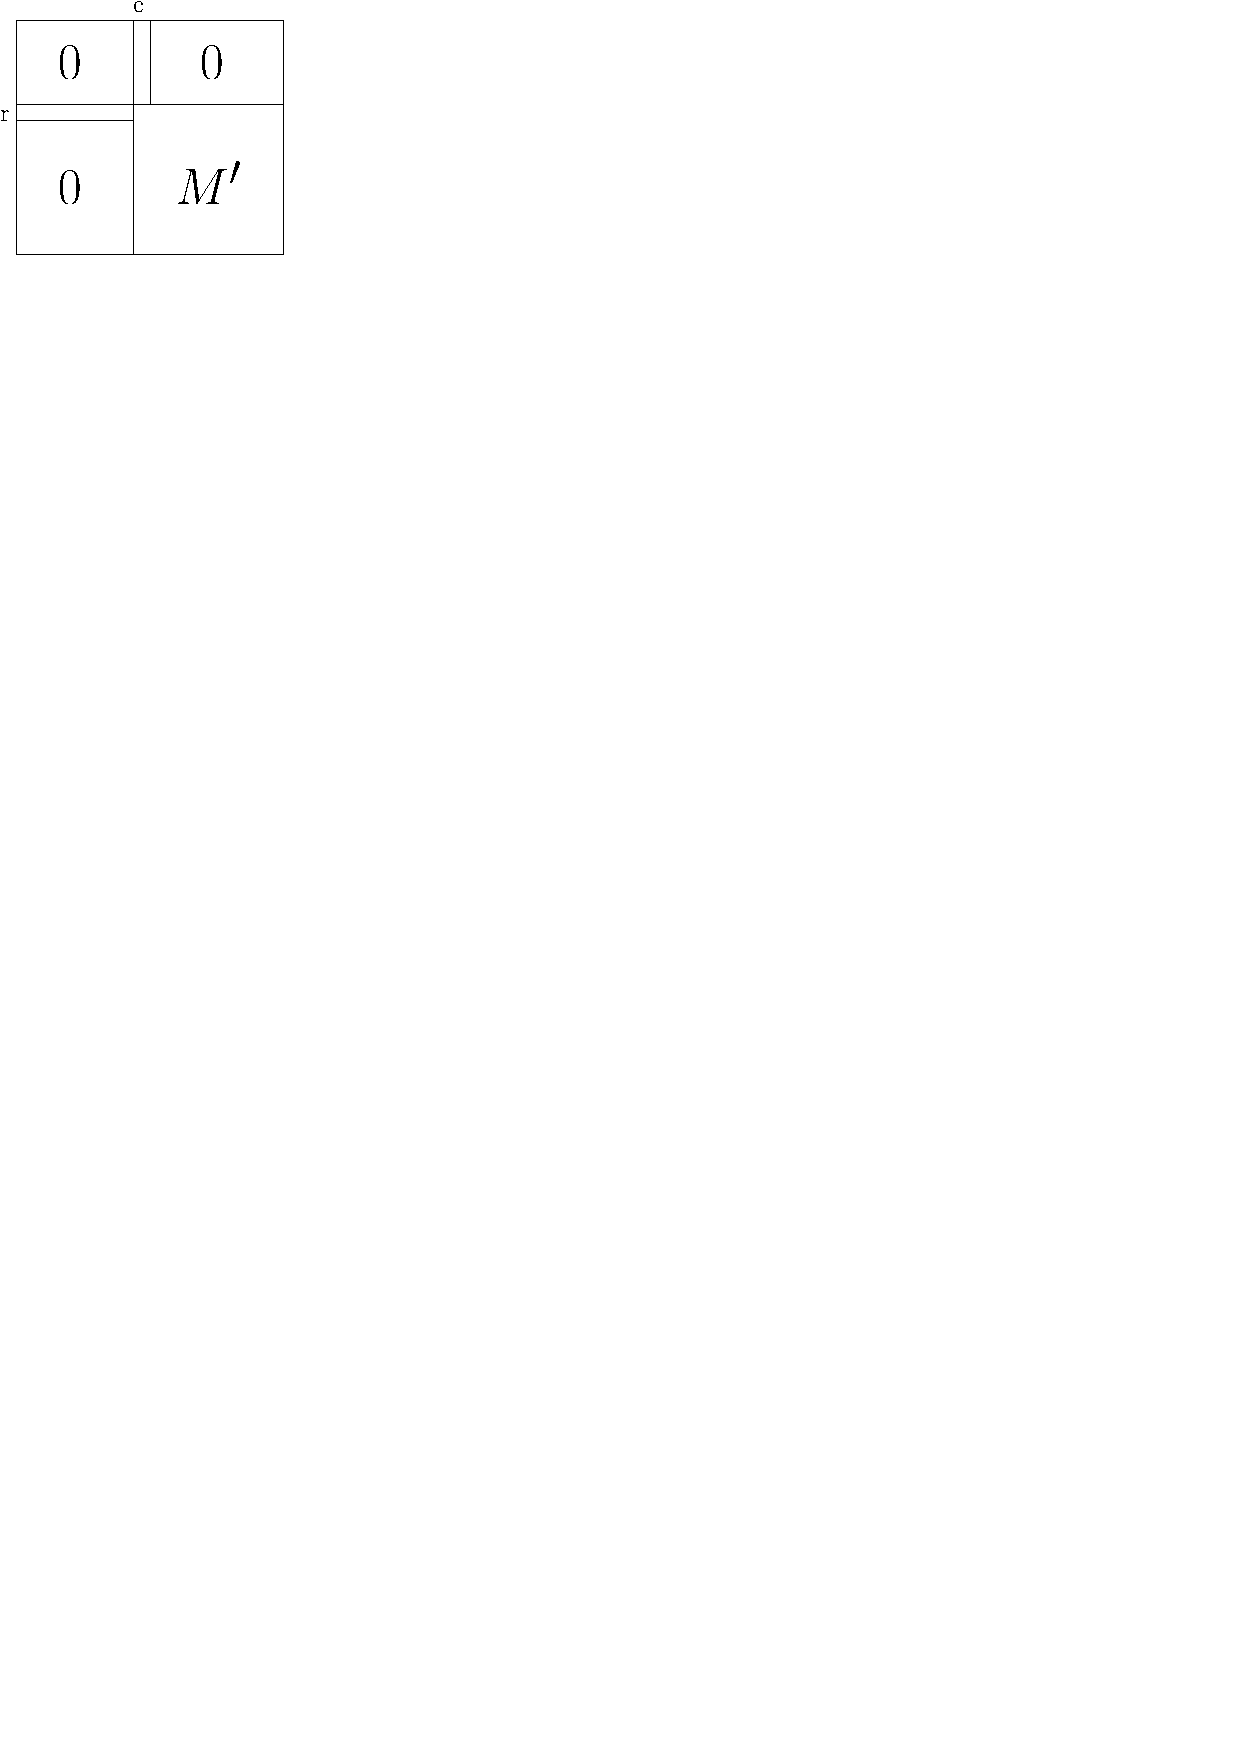
\includegraphics[width=50mm]{img/p12.pdf}
\caption{Characterization of matrices avoiding \usebox{\smlmat} as an interval minor. Matrix $M'$ is a walking matrix.}
\label{fig:p12}
\end{figure}
\begin{proof}
\begin{itemize}
	\item[$\Rightarrow$] If $M$ is a walking matrix then we set $r=c=1$. Otherwise, there are one-entries $M[r,c']$ and $M[r',c]$ such that $r'<r$ and $c'<c$. If there is a one-entry in $M[[r-1],[c-1]],\ M[[r-1],\ [c+1,n]]$ or $M[[r+1,m],[c-1]]$ then $\PimM$. If $M[[r,m],[c,n]]$ is not a walking matrix then it contains $\smm{ &\bullet\\\bullet& }$ and together with $M[r,c']$ it gives us the forbidden pattern.
	\item[$\Leftarrow$] For contradiction, assume that $M$ described in Figure~\ref{fig:p12} contains $P_3$ as an interval minor. Without loss of generality we can assume $P_3[1,1]$ is mapped to the $r$-th row. But then both $P_3[1,2]$ and $P_3[2,1]$ need to be mapped to $M'$ which is a contradiction with it being a walking matrix.
\end{itemize}
\end{proof}

\begin{prop}
For all matrices $M$: $P_4\nim M\Leftrightarrow$ for the top-left most reverse walk~$w$ in $M$ such that there are no one-entries underneath it and for every one-entry $M[r,c]$ on $w$ it holds $M[[r-1],[c-1]]$ is a walking matrix.
\end{prop}
\begin{proof}
\begin{itemize}
	\item[$\Rightarrow$] For contradiction assume there are $r,c$ such that $M[r,c]$ is a one-entry of $w$ and $M[[r-1],[c-1]]$ is not a walking matrix. It means that $\smm{ &\bullet\\\bullet& }\im M[[r-1],[c-1]]$ and together with $M[r,c]$ it gives us the forbidden pattern and a contradiction.
	\item[$\Leftarrow$] For contradiction let $P_4\im M$ and consider a mapping of $P_4$, where $P_4[3,3]$ is mapped to $M[r,c]$ and there is no other one-entry in $M[[r,m],[c,n]]$. Clearly, $M[r,c]$ cannot lie on $w$, because then $M[[r],[c]]$ is a walking matrix and so $M[r,c]$ cannot be used to map $P_4[3,3]$. So $M[r,c]$ lies above $w$ but that is a contradiction with $w$ being top-left most reverse walk in $M$ without one-entries underneath it.
\end{itemize}
\end{proof}

\begin{prop}
For all matrices $M$: $P_5\nim M\Leftrightarrow M=M_1\hsum M_2$ where $\smm{\bullet& \\ &\bullet}\nim M_1$ and $\smm{ &\bullet\\\bullet& }\nim M_2$.
\end{prop}
\begin{proof}
\begin{itemize}
	\item[$\Rightarrow$] Let $e=[r,c]$ be the top-most one-entry of $M$. If $\smm{\bullet& \\ &\bullet}\im M[[m],[c-1]]$, together with $e$ it forms $P_5$. If $\smm{ &\bullet\\\bullet& }\nim M[[m],[c,n]]$ then we are done. Let us assume it is not the case and let $e_{1,1},\ e_{2,2}$ be any two one-entries forming the forbidden pattern. Symmetrically, let $\smm{\bullet& \\ &\bullet}\im M[[m],[c]]$ and let $e_{1,2},\ e_{2,1}$ be any two one-entries forming the forbidden pattern. If we take $e_{1,1},\ e_{1,2}$ and $e_{2,1}$ or $e_{2,2}$ with bigger row, we get $P_5$ as an interval minor of $M$. 
	\item[$\Leftarrow$] For contradiction, let us assume $P_5\im M$. Let us look at the one-entry of $M$ where $P_5[2,2]$ is mapped. If it is in $M_1$ then $\smm{\bullet& \\ &\bullet}\im M_1$ and we get a contradiction. Otherwise we have $\smm{ &\bullet\\\bullet& }\im M_2$ which is again a contradiction.
\end{itemize}
\end{proof}

\begin{prop}
For all matrices $M$: $P_6\nim M\Leftrightarrow$ for the top-right most walk~$w$ in $M$ such that there are no one-entries underneath it and for every one-entry $M[r,c]$ on $w$ there is at most one non-empty column in $M[[r-1],[c+1,n]]$.
\end{prop}
\begin{proof}
\begin{itemize}
	\item[$\Rightarrow$] For contradiction assume that there is a one-entry of the walk $M[r,c]$ for which there are two non-empty columns in $M[[r-1],[c+1,m]]$. Then a one-entry from each of those columns and a one-entry in $M[r,c]$ together give us $P_6\im M$ and a contradiction. 
	\item[$\Leftarrow$] For contradiction let $P_6\im M$. Without loss of generality $P_6[2,1]$ is mapped $M[r,c]$ which lies on $w$. But then $\smm{\bullet&\bullet}\im M[[r-1],[c+1,n]]$ which is a contradiction with it having one-entries in at most one column.
\end{itemize}
\end{proof}

\section{Patterns having four one-entries}
\label{sec:4ones}
These are some of the patterns having four one-entries and no empty lines that we did not characterize so far:
$$P_7=\smm{\bullet&\bullet\\\bullet&\bullet}\ \ \ P_8=\smm{\bullet&\bullet&\bullet\\ &\bullet& }\ \ \ P_9=\smm{ &\bullet& & \\\bullet& & & \\ & & &\bullet\\ & &\bullet& }$$

\begin{lemma}
\label{lemma:p33}
For any matrix $M$: $P_7\nim M\Rightarrow$ there exist integers $r,c$ such that $M[r,c]$ is either
\begin{enumerate}
\item a one-entry and $(r,c)\in\{(1,1),(1,n),(m,1),(m,n)\}$ or
\item top-left empty and bottom-right empty and $(r,c)\not\in\{(1,n),(m,1)\}$ or
\item top-right empty and bottom-left empty and $(r,c)\not\in\{(1,1),(m,n)\}$.
\end{enumerate}
\end{lemma}
\begin{proof}
If there is a one-entry in any corner then we are done. Otherwise, consider $M[1,2]$. It is trivially bottom-left empty and there is no one-entry in the first row of $M$ we are done. Therefore, let $M[1,c_t]$ be the left-most one-entry in the first row. Symmetrically, let $M[m,c_b]$ be the right-most one-entry in the last row, let $M[r_l,1]$ be the bottom most one-entry in the first column and let $M[r_r,n]$ be the top-most one-entry in the last column. It cannot happen that $c_t<c_b$ and $r_r>r_l$, because then $P_7\im M$. Symmetrically, it does not hold at the same time $c_t>c_b$ and $r_r<r_l$. Without loss of generality, let $c_t\geq c_b$ and $r_r\geq r_l$. Matrix $M[[r_r-1],[c_t+1,n]]$ is empty; otherwise, any one-entry there, together with $M[1,c_t],M[m,c_b]$ and $M[r_r,1]$ forms the forbidden pattern. Similarly, matrix $M[[r_r+1,m],[c_t-1]]$ is also empty. Thus $M[r_t,c_t]$ is top-right and bottom-left empty and it is not a corner, because those are empty.
\end{proof}

\begin{prop}
\label{prop:p33}
For all matrices $M$: $P_7\nim M\Leftrightarrow M$ looks like one of the matrices in Figure~\ref{fig:p33}, where $\smm{\bullet&\bullet\\\bullet& }\nim M_1$, $\smm{ &\bullet\\\bullet&\bullet}\nim M_2$, $\smm{\bullet&\bullet\\ &\bullet}\nim M_3$ and $\smm{\bullet& \\\bullet&\bullet}\nim M_4$.
\end{prop}
\begin{figure}[!ht]
\centering
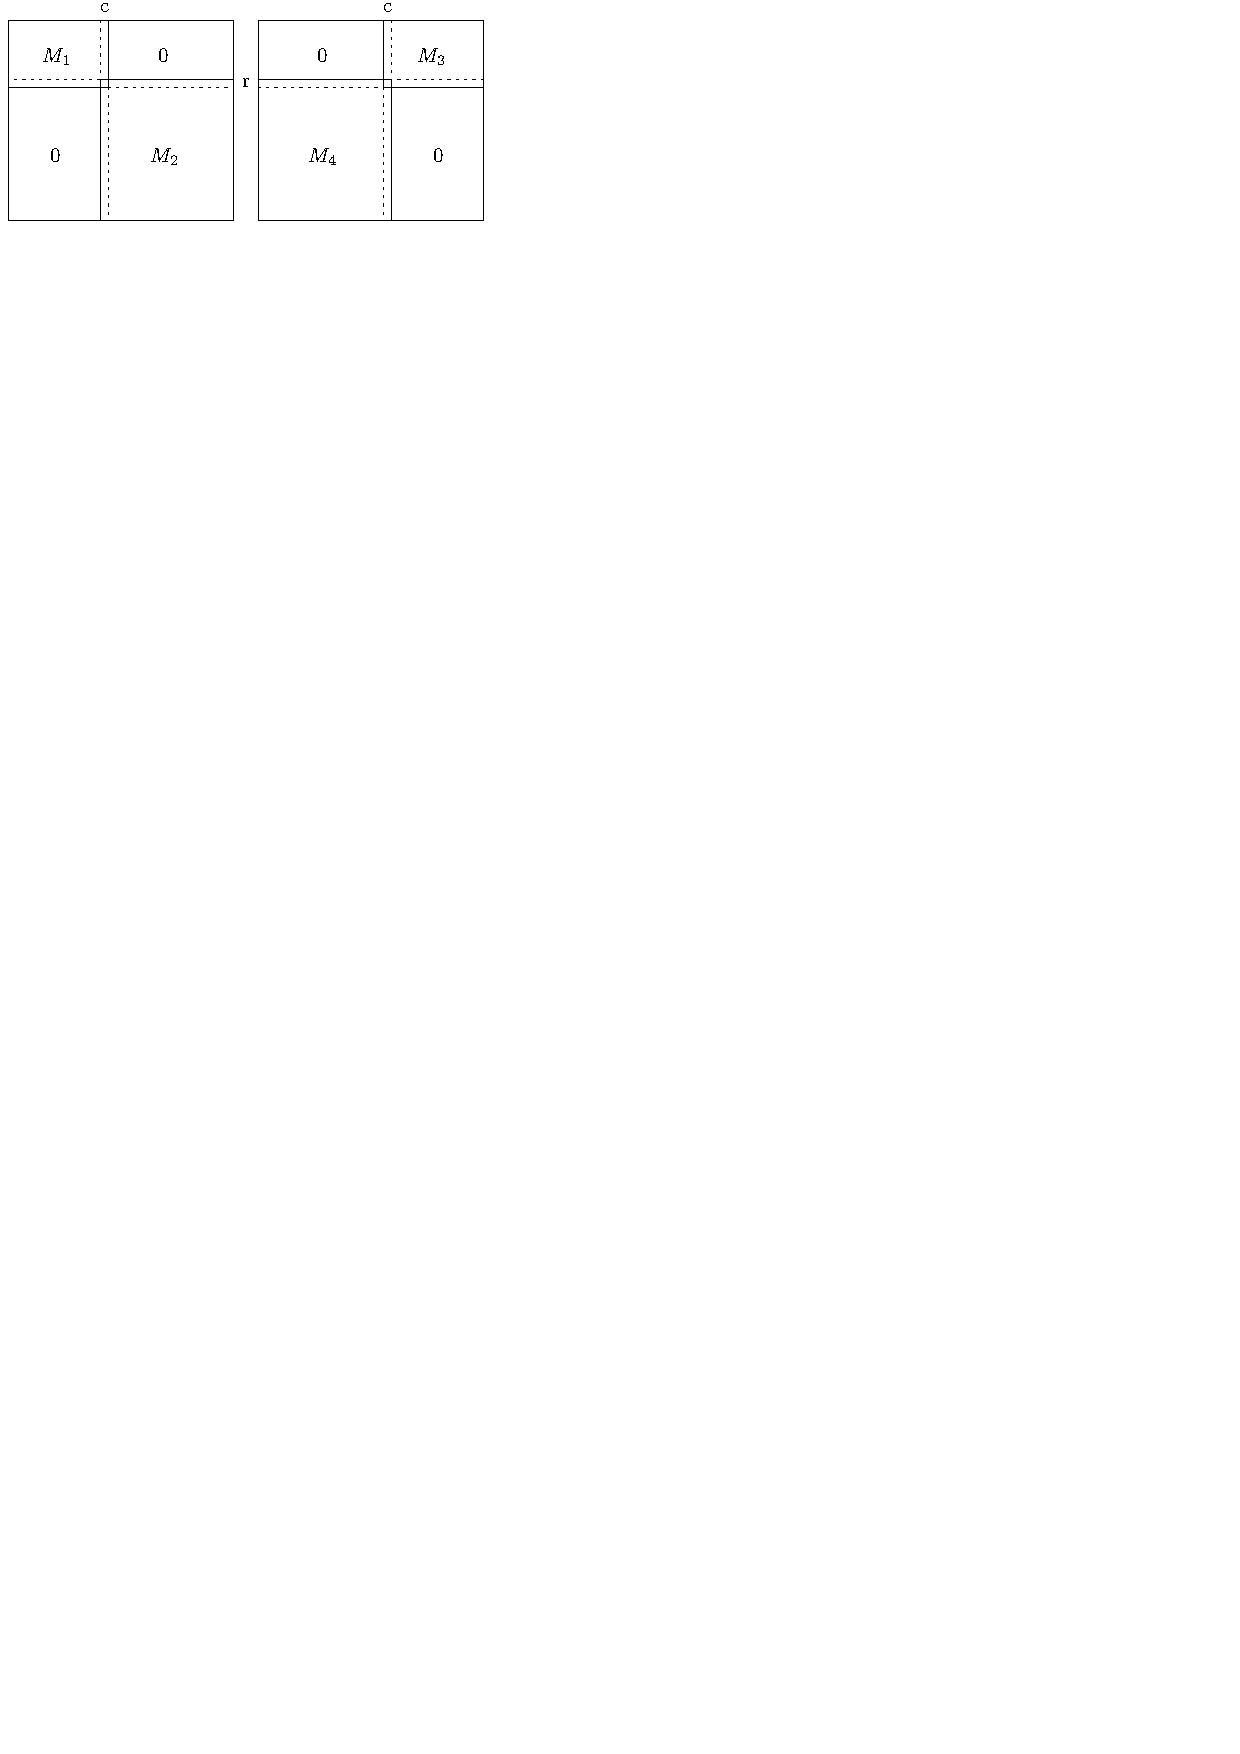
\includegraphics[width=100mm]{img/p33.pdf}
\caption{Characterization of matrices avoiding \usebox{\smlmatb} as an interval minor.}
\label{fig:p33}
\end{figure}
\begin{proof}
\begin{itemize}
	\item[$\Rightarrow$] We proceed by induction on the size of $M$.

If $M\in\bin^{2\times2}$ then it either avoids $\smm{ &\bullet\\\bullet&\bullet}$ or $\smm{\bullet&\bullet\\\bullet& }$ and we are done.

For bigger $M$, from Lemma~\ref{lemma:p33}, there is $M[r,c]$ satisfying some conditions. If there is a one-entry in any corner, we are done because the matrix cannot contain one of the rotations of $\smm{\bullet&\bullet\\\bullet& }$. Otherwise, assume $M[r,c]$ is both top-right and bottom-left empty and $(r,c)\not\in\{(1,n),(m,1)\}$. Let $M_1=M[[r],[c]]$ and $M_2=M[[r,m],[c,n]]$. If $M_1$ is non-empty, then $\smm{ &\bullet\\\bullet&\bullet}\nim M_2$. Symmetrically, $\smm{\bullet&\bullet\\\bullet& }\nim M_1$ if $M_2$ is non-empty. If one of them is empty, the other is a smaller matrix avoiding $P$ as an interval minor and the statement follows from the induction.
	\item[$\Leftarrow$] Without loss of generality, let us assume $M$ looks like the left matrix in Figure~\ref{fig:p33}. For contradiction, assume $\PimM$. In that case, we can partition $M$ into four quadrants such that there is at least one one-entry in each of them. It does not matter where we partition it, every time we either get $\smm{\bullet&\bullet\\\bullet& }\im M_1$ or $\smm{ &\bullet\\\bullet&\bullet}\im M_2$, which is a contradiction.
\end{itemize}
\end{proof}

\begin{lemma}
\label{lemma:p72}
For all matrices $M$: $P_8\nim M\Rightarrow M=M_1\hsum M_2$ where
\begin{enumerate}
\item $\smm{\bullet&\bullet\\ &\bullet}\nim M_1$ and $\smm{ &\bullet\\\bullet& }\nim M_2$ or
\item $\smm{\bullet& \\ &\bullet}\nim M_1$ and $\smm{\bullet&\bullet\\\bullet& }\nim M_2$.
\end{enumerate}
\end{lemma}
\begin{proof}
Let $e=[r,c]$ be the top-most one-entry of $M$. If $\smm{\bullet&\bullet\\ &\bullet}\im M[[m],[c-1]]$, together with $e$ it would be the whole $P_8$. Symmetrically, $\smm{\bullet&\bullet\\\bullet& }\nim M[[m],[c+1,n]]$. For contradiction assume $\smm{\bullet& \\ &\bullet}\im M[[m],[c]]$ and let $e_{1,1},\ e_{2,2}$ (none of them equal to $e$) be any two one-entries forming the pattern. Symmetrically, assume $\smm{ &\bullet\\\bullet& }\im M[[m],[c,n]]$ and let $e_{1,2},\ e_{2,1}$ be any two one-entries forming the pattern. Then $e_{1,1},\ e,\ e_{1,2}$ and $e_{2,1}$ or $e_{2,2}$ with bigger row give us mapping of $P_8$ to $M$.
\end{proof}

\begin{prop}
\label{prop:p72}
For all matrices $M$: $P_8\nim M\Leftrightarrow M$ is structured like the matrix in Figure~\ref{fig:p72} where $\smm{\bullet& \\ &\bullet}\nim M_1$ and $\smm{ &\bullet\\\bullet& }\nim M_2$.
\end{prop}
\begin{figure}[!ht]
\centering
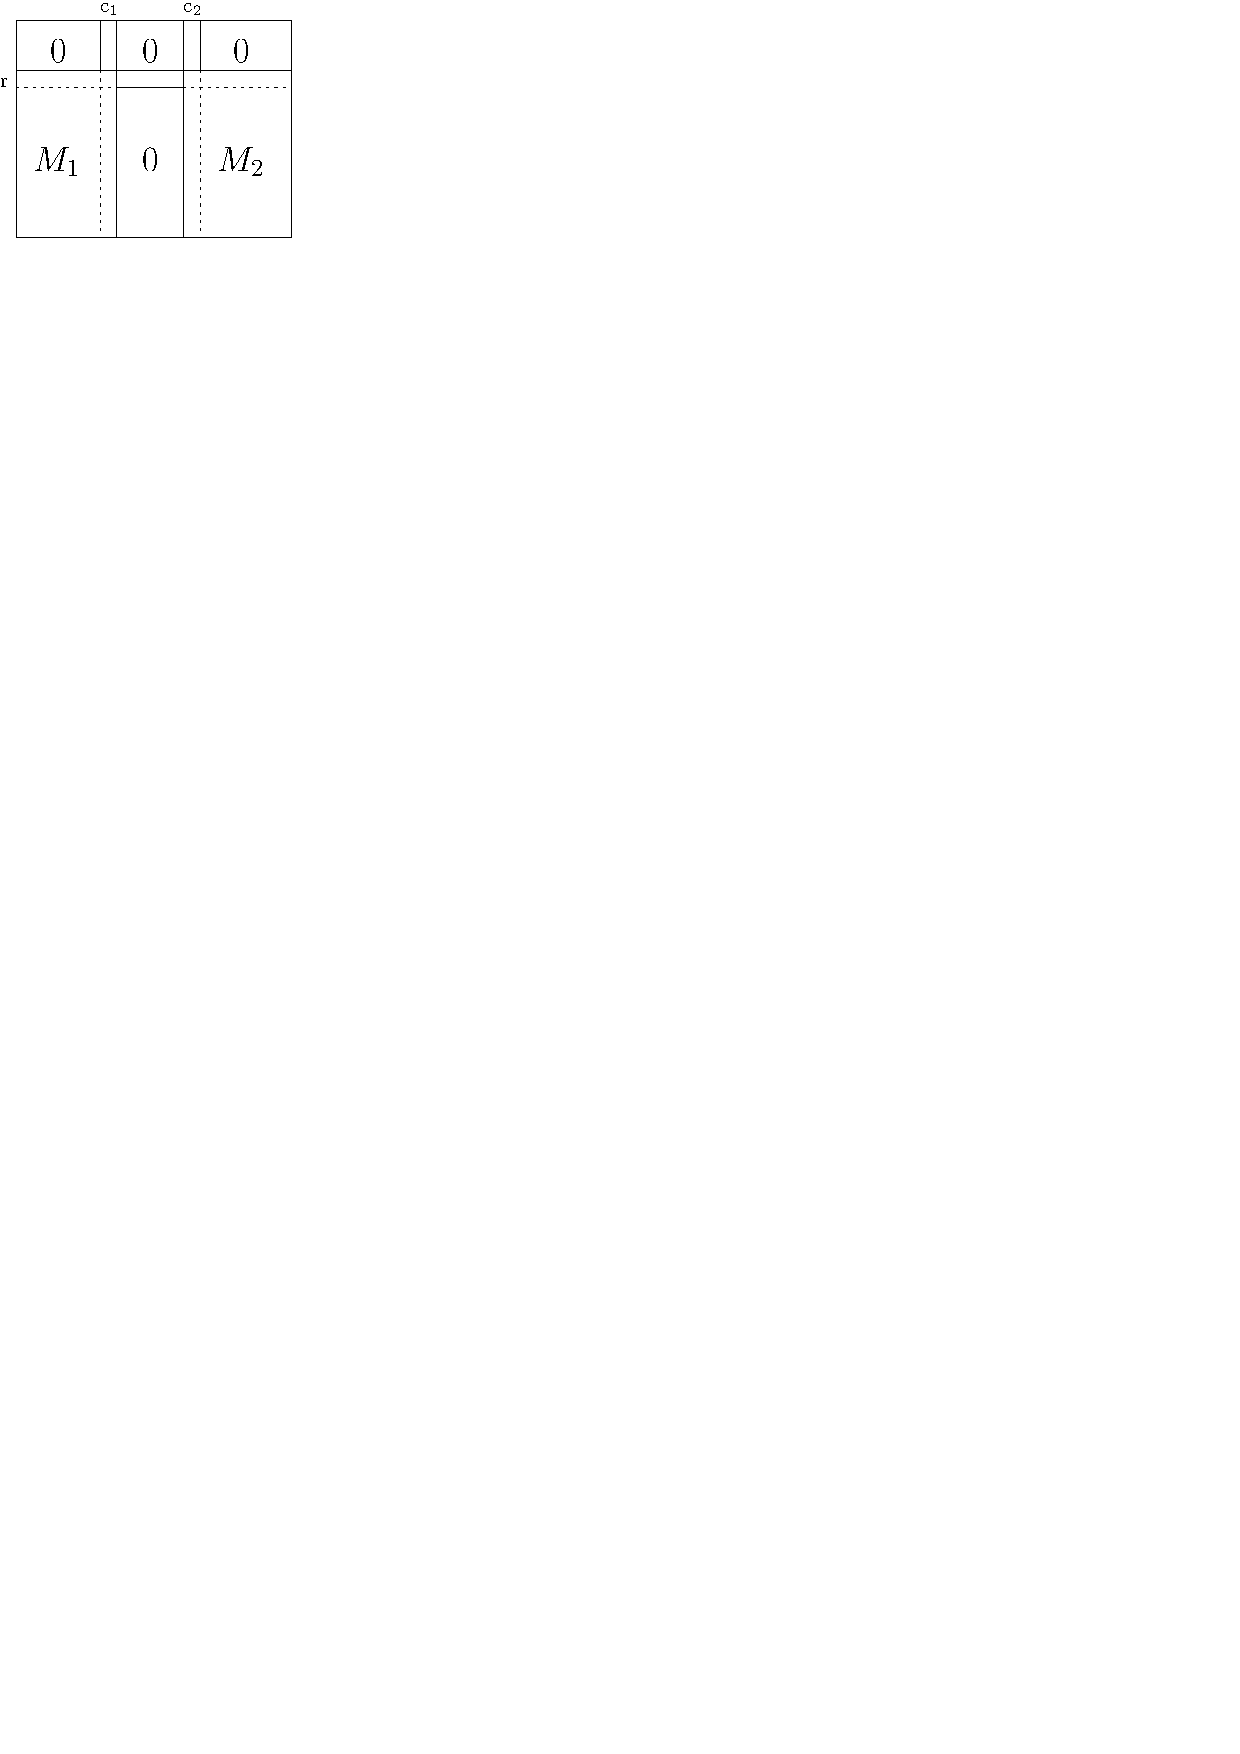
\includegraphics[width=60mm]{img/p72.pdf}
\caption{Characterization of matrices avoiding \usebox{\smlmatc} as an interval minor.}
\label{fig:p72}
\end{figure}
\begin{proof}
\begin{itemize}
	\item[$\Rightarrow$] From Lemma~\ref{lemma:p72} we know $M=M_1'\hsum M_2'$ where $\smm{\bullet&\bullet\\ &\bullet}\nim M_1'$ and $\smm{ &\bullet\\\bullet& }\nim M_2'$. The second case can be dealt with symmetrically. From Proposition~\ref{prop:p31} we have that $M_1'$ can be characterized exactly like $M[[m],[c_2-1]$ and $M[[m],[c_2,n]]$ forms a walking matrix. If there are two different columns having a one-entry above the $r$-th row, together with a one-entry in the $r$-th row between the columns $c_1$ and $c_2$ and a one-entry in the $c_1$-th column above the $r$-th row they form a mapping of $P_8$.
	\item[$\Leftarrow$] One-entry $P_8[2,2]$ can not be mapped anywhere but to the $r$-th row, but in that case there are at most two columns having one-entries above it.
\end{itemize}
\end{proof}

\section{Multiple patterns}

\begin{prop}
\label{prop:twopatterns}
Let $P_{10}=\smm{\circ&\circ&\bullet\\\bullet&\circ&\circ}$ and $P_{11}=\smm{\circ&\bullet\\\circ&\circ\\\bullet&\circ}$, then for all matrices $M$: $\{P_{10},P_{11}\}\nim M\Leftrightarrow$ for the top-right most walk~$w$ in $M$ such that there are no one-entries underneath it each one-entry $M[r,c]$ is either on $w$ or both $M[r+1,c]$ and $M[r,c-1]$ are on $w$.
\end{prop}
\begin{proof}
\begin{itemize}
	\item[$\Rightarrow$] For contradiction assume there is a one-entry anywhere but on $w$ or directly diagonally above any bottom-left corner of $w$. Then this one-entry together with at least one bottom-left corner of $w$ give us $P_{10}$ or $P_{11}$ and a contradiction.
	\item[$\Leftarrow$] If we take any one-entry~$e$, from the description of $M$ there is no one-entry that creates $P_{10}$ or $P_{11}$ with $e$.
\end{itemize}
\end{proof}